% Fig 1 (hero); panels (a, grids) and (b) from scripts/gen_fig1*.py, schematic drawn in fig1a_schematic.tex
\begin{figure*}[t]
  \centering
  % Fig 1a schematic: CNN -> bottleneck z -> 8-qubit VQC head -> linear readout, and the common
% linear probe on the frozen bottleneck. Requires tikz with positioning, arrows.meta, fit,
% shapes.geometric.
\begin{tikzpicture}[
    x=1cm, y=1cm, font=\footnotesize,
    box/.style={draw, rounded corners=1.5pt, minimum height=6mm, inner sep=2.5pt, align=center},
    gate/.style={draw, fill=white, minimum height=4.4mm, minimum width=9mm, inner sep=1pt, font=\scriptsize},
    arr/.style={-{Stealth[length=1.6mm]}, semithick},
  ]
  % classical front end
  \node[box] (img) at (0, 0) {image};
  \node[box, trapezium, trapezium angle=70, shape border rotate=270, minimum width=8mm] (cnn) at (1.45, 0) {CNN};
  \node[box] (z) at (2.95, 0) {$z\in\mathbb{R}^8$};
  \draw[arr] (img) -- (cnn);
  \draw[arr] (cnn) -- (z);
  \draw[arr] (z.east) -- (3.95, 0);

  % qubit wires q0, q1, ..., q7
  \foreach \y/\lab in {0.62/q_0, 0.22/q_1, -0.62/q_7} {
    \draw[thin] (4.55, \y) -- (10.0, \y);
    \node[font=\scriptsize, anchor=east] at (4.55, \y) {$\lab$};
  }
  \foreach \x in {5.15, 6.75, 9.45} \node[font=\scriptsize] at (\x, -0.18) {$\vdots$};

  % encoding R_y(a_j)
  \foreach \y/\j in {0.62/0, 0.22/1, -0.62/7}
    \node[gate, fill=blue!6] at (5.15, \y) {$R_y(a_{\j})$};

  % one variational layer: R_y R_z on every qubit, then a CNOT ring; repeated L times
  \foreach \y in {0.62, 0.22, -0.62}
    \node[gate] at (6.75, \y) {$R_y R_z$};
  \fill (7.65, 0.62) circle (1.3pt);                       % CNOT(0 -> 1)
  \draw (7.65, 0.62) -- (7.65, 0.22);
  \draw (7.65, 0.22) circle (2.6pt); \draw (7.65, 0.13) -- (7.65, 0.31);
  \fill (8.0, 0.22) circle (1.3pt);                        % CNOT(1 -> 2), down the ring
  \draw (8.0, 0.22) -- (8.0, -0.08);
  \node[font=\scriptsize] at (8.0, -0.2) {$\cdots$};
  \fill (8.4, -0.62) circle (1.3pt);                       % CNOT(7 -> 0) closes the ring
  \draw (8.4, -0.62) -- (8.4, 0.62);
  \draw (8.4, 0.62) circle (2.6pt); \draw (8.4, 0.53) -- (8.4, 0.71);
  \draw[dashed, rounded corners=2pt, gray] (6.15, -0.88) rectangle (8.65, 0.88);
  \node[font=\scriptsize, gray!70!black, anchor=north] at (7.4, -0.9) {$\times L$; CNOT layout varied};

  % measurement
  \foreach \y/\k in {0.62/0, 0.22/1, -0.62/7}
    \node[gate, minimum width=8mm] at (9.45, \y) {$\langle Z_{\k}\rangle$};

  % head frame and readout
  \node[draw, dashed, rounded corners=3pt, fit={(3.95, 1.0) (9.95, -1.25)}, inner sep=1pt,
        label={[font=\scriptsize, anchor=south west]north west:VQC head, 8 qubits}] (head) {};
  \node[box, anchor=west] (lin) at (10.75, 0) {Linear};
  \draw[arr] (10.0, 0) -- (lin.west);

  % zero-rotation identity
  \node[font=\scriptsize, anchor=west] at (4.25, -1.65)
    {$a_j=\pi\tanh z_j$;\ \ at zero variational rotations
     $\langle Z_k\rangle=\prod_{j\in S_k}\cos a_j$, with $S_k$ fixed by the CNOTs};

  % common linear probe on the frozen bottleneck
  \node[box, draw=gray, text=gray!70!black] (probe) at (2.55, -1.5) {common linear probe\\[-1pt](backbone frozen)};
  \draw[arr, dashed, gray] (z) -- (probe);
\end{tikzpicture}
\\[3mm]
  \begin{minipage}[c]{0.36\textwidth}
    \centering
    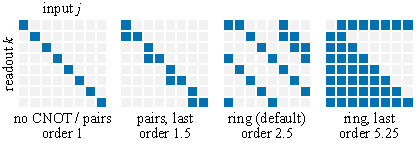
\includegraphics[width=\linewidth]{figures/fig1a_supports.pdf}\\[1mm]
    {\small (a)}
  \end{minipage}\hfill
  \begin{minipage}[c]{0.60\textwidth}
    \centering
    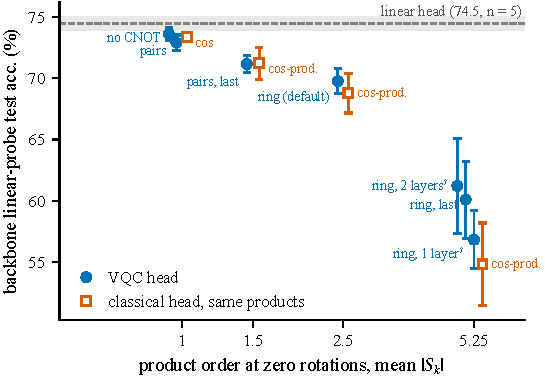
\includegraphics[width=\linewidth]{figures/fig1b_probe_vs_order.pdf}\\
    {\small (b)}
  \end{minipage}
  \caption{\textbf{(a)} A CNN feeds an 8-dimensional bottleneck $z$ into an 8-qubit VQC head
  (default: four $R_yR_z$ layers, each followed by a CNOT ring $(q, q{+}1 \bmod 8)$; variants
  place CNOTs after the last layer only (``last''), use $L\in\{1,2\}$ layers, or replace the ring
  by disjoint pairs $(0,1),(2,3),(4,5),(6,7)$). With every variational rotation at zero, each
  readout is exactly $\langle Z_k\rangle=\prod_{j\in S_k}\cos(\pi\tanh z_j)$; the grids mark
  $j\in S_k$ in blue (rows: readouts $k$, columns: inputs $j$). Pairs after every layer cancel
  at zero rotations, so their supports equal the no-CNOT ones. Product order is
  $\frac18\sum_k|S_k|$. The backbone is evaluated by one common linear probe on the frozen
  bottleneck. \textbf{(b)} CIFAR-10 with 4,000 training images: probe test accuracy against
  product order (log axis) for VQC heads (filled) and classical heads trained end to end on the
  zero-rotation products of a circuit (open; at order 5.25 these are the supports of ``ring,
  last'' and ``ring, 1 layer''; ``ring, 2 layers'' has different supports of the same mean
  order). Mean $\pm$ SD over 5 seeds ($\dagger$: 3); head learning rate selected on mean
  validation accuracy over seeds 0--2, seeds 3--4 run at that choice. Dashed line and band:
  linear head. Points at one order are offset horizontally. The plot shows an association;
  order co-varies with support overlap. Open diamonds: six CNOT layouts outside the ring family (5 seeds, \cref{app:family}),
  whose probe accuracy was predicted before training from the dotted fit over the ring-family (seeds 0--2)
  VQC circuits (linear in order, hence curved on the log axis); brickwork lies 5 points above its prediction. Open triangles: a CZ ring (entangling, order 1) and the CNOT-free circuit read out with $Z_kZ_{k+1}$ or $Z_kZ_{k+1}Z_{k+2}$ (orders 2 and 3), pre-registered, 5 seeds (\cref{tab:generality}).}
  \label{fig:hero}
\end{figure*}
